\section{The Ornstein-Uhlenbeck Process}

We now consider one of the most important stochastic processes in science and engineering: the \textbf{Ornstein-Uhlenbeck (OU) process}. It appears in numerous contexts, from describing the velocity of a particle in a fluid (the original Langevin model) to modeling the voltage in a noisy electronic circuit. In essence, it is the canonical model for any noisy, linear system that tends to return to an equilibrium state.

The general form of the OU process is given by the SDE:
$$
dz = -\gamma z\,dt + \omega\,dW
$$
where $\gamma > 0$ is the \textit{drift} or \textit{relaxation rate}, which constantly pulls the process back towards its mean (in this case, zero), and $\omega$ is the noise intensity. This linear restoring force is what distinguishes the OU process from the free-wandering Wiener process.

\subsubsection{Solving the Ornstein-Uhlenbeck SDE}

To solve this linear SDE, we can use a technique analogous to the integrating factor method for ODEs. We define a new variable $Q(t) = e^{\gamma t}z(t)$. Our goal is to find an SDE for $Q(t)$. Using Ito's product rule (or Ito's lemma on $\psi(z,t) = e^{\gamma t}z$), we find:
\begin{align*}
    dQ &= (d(e^{\gamma t}))z + e^{\gamma t}(dz) \\
    &= (\gamma e^{\gamma t}dt)z + e^{\gamma t}(-\gamma z\,dt + \omega dW(\tau)) \\
    &= \gamma e^{\gamma t}z\,dt - \gamma e^{\gamma t}z\,dt + \omega e^{\gamma t}dW(\tau) \\
    &= \omega e^{\gamma t}dW(\tau)
\end{align*}
The drift terms have canceled perfectly, leaving a very simple SDE for $Q(t)$. We can now integrate it from 0 to $t$:
$$
Q(t) - Q(0) = \omega \int_0^t e^{\gamma \tau}dW(\tau) \quad \implies \quad Q(t) = Q(0) + \omega \int_0^t e^{\gamma \tau}dW(\tau)
$$
Substituting back $z(t) = e^{-\gamma t}Q(t)$ and $z(0) = Q(0)$, we arrive at the solution for the Ornstein-Uhlenbeck process:
$$
z(t) = z(0)e^{-\gamma t} + \omega \int_0^t e^{\gamma(\tau-t)}dW(\tau)
$$
The solution consists of two parts: a deterministic decay of the initial condition, $z(0)e^{-\gamma t}$, and a stochastic integral that represents the accumulated effect of the noise, with past noise contributions being exponentially "forgotten" over time due to the $e^{\gamma(\tau-t)}$ term.

\subsubsection{Statistical Properties}

From the solution, we can derive the key statistical properties of the OU process.

\begin{itemize}
    \item \textbf{Mean}

    Since the stochastic integral $\int e^{\gamma(\tau-t)}dW(\tau)$ has zero mean, the mean of the process is simply the deterministic part:
    $$
    \boxed{\langle z(t) \rangle = \langle z(0) \rangle e^{-\gamma t}}
    $$
    Assuming a deterministic starting point $z(0)$, the mean exponentially decays to zero, which is the equilibrium point of the system.

    \item \textbf{Variance}
    
    The variance calculation is more involved but highly instructive. Starting from our solution:
    $$
    z(t) = z(0)e^{-\gamma t} + \omega \int_0^t e^{\gamma(\tau-t)}dW(\tau)
    $$
    we can calculate the variance by expanding $\text{Var}[z(t)] = \langle z(t)^2 \rangle - \langle z(t) \rangle^2$. Since $\langle z(t) \rangle = z(0)e^{-\gamma t}$ (assuming deterministic initial condition), we have:
    $$
    \text{Var}[z(t)] = \left\langle \left( z(0)e^{-\gamma t} + \omega \int_0^t e^{\gamma(\tau-t)}dW(\tau) \right)^2 \right\rangle - z(0)^2e^{-2\gamma t}
    $$
    Expanding the square:
    \small
    $$
    \text{Var}[z(t)] = \left\langle z(0)^2e^{-2\gamma t} + 2z(0)e^{-\gamma t}\omega \int_0^t e^{\gamma(\tau-t)}dW(\tau) + \omega^2 \left(\int_0^t e^{\gamma(\tau-t)}dW(\tau)\right)^2 \right\rangle - z(0)^2e^{-2\gamma t}
    $$
    \normalsize
    The cross term vanishes since $\langle dW(\tau) \rangle = 0$, leaving:
    $$
    \text{Var}[z(t)] = \omega^2 \left\langle \left(\int_0^t e^{\gamma(\tau-t)}dW(\tau)\right)^2 \right\rangle
    $$
    
    Applying the mean, we get:
    $$
    \text{Var}[z(t)] = \omega^2 \left\langle \left(\int_0^t e^{\gamma(\tau-t)}dW(\tau)\right)^2 \right\rangle = \omega^2 \int_0^t \int_0^t e^{\gamma(\tau-t)}e^{\gamma(s-t)}\langle dW(\tau)dW(s) \rangle
    $$
    Using the property that $\langle dW(\tau)dW(s) \rangle = \delta(\tau - s)d\tau ds$, the double integral becomes:
    $$
    \text{Var}[z(t)] = \omega^2 \int_0^t \int_0^t e^{\gamma(\tau + s -2t)}\delta(s-\tau)\,ds\,d\tau  = \omega^2 \int_0^t e^{2\gamma(\tau-t)}d\tau
    $$
    Evaluating this integral:
    $$
    \text{Var}[z(t)] = \omega^2 e^{-2\gamma t} \int_0^t e^{2\gamma\tau}d\tau = \omega^2 e^{-2\gamma t} \left[ \frac{e^{2\gamma\tau}}{2\gamma} \right]_0^t = \frac{\omega^2}{2\gamma}(1 - e^{-2\gamma t})
    $$

    The total variance becomes:
    $$
    \boxed{\text{Var}[z(t)] = \text{Var}[z(0)]e^{-2\gamma t} + \frac{\omega^2}{2\gamma}(1 - e^{-2\gamma t})}
    $$
    As $t \to \infty$, the first term vanishes, and the variance approaches a constant stationary value:
    $$
    \lim_{t\to\infty} \text{Var}[z(t)] = \frac{\omega^2}{2\gamma}
    $$
    This is a crucial difference from the Wiener process, whose variance grows linearly and without bound. The restoring force in the OU process balances the diffusive effect of the noise, leading to a finite stationary variance.

    \item \textbf{Autocovariance}

    The autocovariance function for times $t$ and $q$ is defined as:
    $$
    C(t,q) = \langle (z(t) - \langle z(t) \rangle)(z(q) - \langle z(q) \rangle) \rangle
    $$
    For simplicity, let's assume the process starts at $z(0) = 0$. In this case, the mean is $\langle z(t) \rangle = 0$ for all $t$, so the autocovariance is simply the autocorrelation: $C(t,q) = \langle z(t)z(q) \rangle$.

    Using the solution for $z(t)$ with $z(0)=0$:
    $$
    z(t) = \omega \int_0^t e^{\gamma(s-t)}dW(s)
    $$
    The autocorrelation is:
    \small
    \begin{align*}
        \langle z(t)z(q) \rangle &= \left\langle \left( \omega \int_0^t e^{\gamma(s-t)}dW(s) \right) \left( \omega \int_0^q e^{\gamma(\tau-q)}dW(\tau) \right) \right\rangle \\
        &= \omega^2 e^{-\gamma(t+q)} \left\langle \int_0^t e^{\gamma s}dW(s) \int_0^q e^{\gamma \tau}dW(\tau) \right\rangle \\
        &= \omega^2 e^{-\gamma(t+q)} \int_0^t \int_0^q e^{\gamma(s+\tau)} \langle dW(s)dW(\tau) \rangle
    \end{align*}
    \normalsize
    Using the property $\langle dW(s)dW(\tau) \rangle = \delta(s-\tau)ds\,d\tau$, the double integral collapses into a single integral. We must evaluate the integral over the domain $[0,t] \times [0,q]$.
    $$
    \langle z(t)z(q) \rangle = \omega^2 e^{-\gamma(t+q)} \int_0^t \int_0^q \, e^{\gamma(\tau + s)} \delta(\tau - s) d\tau ds
    $$
    
For the evaluation of this integral, we need to consider two cases:

    \begin{itemize}
        \item \textbf{Case 1: $t \leq q$}
        
        When $t \leq q$, the domain of integration is restricted by the smaller upper limit. The delta function $\delta(\tau - s)$ forces $\tau = s$, so we integrate over the overlap region $[0, t]$:
        $$
        \langle z(t)z(q) \rangle = \omega^2 e^{-\gamma(t+q)} \int_0^t e^{2\gamma s} ds
        $$

        \vspace{-0.5em}

        Evaluating the integral:
        $$
        \langle z(t)z(q) \rangle = \omega^2 e^{-\gamma(t+q)} \left[ \frac{e^{2\gamma s}}{2\gamma} \right]_0^t = \frac{\omega^2}{2\gamma} e^{-\gamma(t+q)} (e^{2\gamma t} - 1)
        = \frac{\omega^2}{2\gamma} \left( e^{-\gamma(q-t)} - e^{-\gamma(q+t)} \right)
        $$

        \item \textbf{Case 2: $t > q$}
        
        When $t > q$, we integrate over $[0, q]$:
        $$
        \langle z(t)z(q) \rangle = \omega^2 e^{-\gamma(t+q)} \int_0^q e^{2\gamma s} ds = \frac{\omega^2}{2\gamma} \left( e^{-\gamma(t-q)} - e^{-\gamma(t+q)} \right)
        $$
    \end{itemize}

    Combining both cases, we can write the autocorrelation function as:
    $$
    \boxed{\langle z(t)z(q) \rangle = \frac{\omega^2}{2\gamma} \left( e^{-\gamma|t-q|} - e^{-\gamma(t+q)} \right)}
    $$
    For a stationary process (when $t, q \to \infty$), the second term vanishes, and we obtain the stationary autocorrelation function:
    $$
    R_z(\tau) = \lim_{t \to \infty} \langle z(t)z(t + \tau) \rangle = \frac{\omega^2}{2\gamma} e^{-\gamma|\tau|}
    $$
    where $\tau = |t-q|$ is the time lag. This autocorrelation decays exponentially with a characteristic time $1/\gamma$. In the limit of rapid relaxation ($\gamma \to \infty$), the autocorrelation function becomes sharply peaked and tends toward a Dirac delta function.
\end{itemize}

We introduce now a scaling relation between the noise intensity and the relaxation rate, by setting:
$$
\omega = c\,\gamma
$$
with $c$ a constant. Under this scaling, the SDE for $z$ becomes
$$
\dot{z} = -\gamma\,z + c\,\gamma\,\xi(t).
$$

The autocorrelation function for $z$ then reads
$$
R_z(h) = \frac{c^2}{2}\,\gamma\,e^{-\gamma|h|}, \qquad R_z(0) = \frac{c^2}{2}\,\gamma.
$$
Its total area is given by
$$
\int_{-\infty}^{+\infty} R_z(h)\,dh 
=
\int_{-\infty}^{+\infty} \frac{c^2}{2}\,\gamma\,e^{-\gamma|h|}\,dh.
=
\frac{c^2}{2}\,\gamma \cdot \frac{2}{\gamma} = c^2.
$$

For small characteristic times ($\tau=1/\gamma$ small), the autocorrelation function $R_z(h)$ approximates a white noise process:
$$
\lim_{\gamma \to \infty} R_z(h;\gamma) = c^2\,\delta(h).
$$

This derivation shows how, by choosing the scaling $\omega = c\,\gamma$, the fluctuations in the linearized dynamics around a stable equilibrium effectively become white noise in the fast relaxation limit.

\subsection{The OU Process as a Low-Pass Filter}

One of the most important interpretations of the Ornstein-Uhlenbeck process is as a \textbf{low-pass filter}. It takes a "noisy" input signal (white noise) and produces a smoother, more physically realistic output by attenuating high-frequency fluctuations. To understand this, we can analyze the process in the frequency domain using the Fourier transform.

\subsubsection{The Fourier Transform and Linear Systems}
Let $f(t)$ be a well-behaved function. Its Fourier transform, $\hat{f}(\omega)$, is defined as:
$$
\mathcal{F}[f(t)] = \hat{f}(\omega) = \int_{-\infty}^{+\infty} f(t) e^{-i\omega t} dt
$$
A key property of the Fourier transform, which can be shown using integration by parts, is how it acts on derivatives:
$$
\mathcal{F}[f'(t)] = i\omega \mathcal{F}[f(t)] = i\omega \hat{f}(\omega)
$$
This property turns differentiation in the time domain into multiplication in the frequency domain, which is extremely useful for solving linear differential equations. For example, consider a general first-order linear system with input $y(t)$ and output $f(t)$:
$$
f'(t) + \alpha f(t) = y(t)
$$
Taking the Fourier transform of the entire equation gives:
$$
i\omega\hat{f}(\omega) + \alpha\hat{f}(\omega) = \hat{y}(\omega) \quad \implies \quad \hat{f}(\omega) = \frac{\hat{y}(\omega)}{i\omega + \alpha}
$$
The term $H(\omega) = 1/(i\omega + \alpha)$ is called the \textbf{transfer function} of the system. The power of the output signal is related to the power of the input signal by the squared magnitude of the transfer function:
$$
|\hat{f}(\omega)|^2 = \frac{|\hat{y}(\omega)|^2}{\omega^2 + \alpha^2}
$$

\subsubsection{Power Spectrum of the OU Process}
We can apply this framework to the OU process, which is described by the linear SDE:
$$
\frac{dz}{dt} + \gamma z = \kappa \xi(t)
$$
Taking the Fourier transform, we get:
$$
(i\omega + \gamma)\hat{z}(\omega) = \kappa \mathcal{F}[\xi(t)] \quad \implies \quad \hat{z}(\omega) = \frac{\kappa}{i\omega + \gamma} \mathcal{F}[\xi(t)]
$$
To analyze the filtering effect, we compare the \textbf{power spectral density} of the input signal, $\xi(t)$, with that of the output signal, $z(t)$. The power spectrum is the Fourier transform of the autocorrelation function.

For the input signal (white noise), the autocorrelation is $R_{\xi}(h) = \delta(h)$ (assuming unit variance for simplicity). Its power spectrum is therefore constant:
$$
\mathcal{F}[R_{\xi}(h)] = \mathcal{F}[\delta(h)] = \int_{-\infty}^{+\infty} \delta(h) e^{-i\omega h} dh = 1
$$
This flat spectrum is why it's called "white" noise: it contains equal power at all frequencies $\omega$.

For the output signal, $z(t)$, we previously found its stationary autocorrelation function to be:
$$
R_{z}(h) = \frac{\kappa^2}{2\gamma} e^{-\gamma|h|}
$$
The power spectrum of the output is the Fourier transform of this function:
$$
\mathcal{F}[R_{z}(h)] = \frac{\kappa^2}{2\gamma} \int_{-\infty}^{+\infty} e^{-\gamma|h|} e^{-i\omega h} dh
$$
We can split the integral over positive and negative values of $h$:
$$
= \int_{-\infty}^{0} e^{(\gamma-i\omega)h}dh + \int_{0}^{+\infty} e^{-(\gamma+i\omega)h}dh = \frac{1}{\gamma-i\omega} + \frac{1}{\gamma+i\omega} = \frac{2\gamma}{\gamma^2 + \omega^2}
$$
Substituting this back, we get the output power spectrum:
$$
\mathcal{F}[R_{z}(h)] = \frac{\kappa^2}{2\gamma} \left( \frac{2\gamma}{\gamma^2 + \omega^2} \right) = \frac{\kappa^2}{\gamma^2 + \omega^2}
$$
This function, known as a \textbf{Lorentzian}, is peaked at $\omega=0$ and decays as $1/\omega^2$ for high frequencies. The OU process acts as a low-pass filter: it suppresses high-frequency components of the input white noise while allowing low-frequency components to pass through, resulting in a smoother, more physically plausible random process.

\vspace{-0.5em}
\begin{figure}[H]
    \centering
    \begin{minipage}{0.45\textwidth}
    \centering
    % Input graph: a constant function
    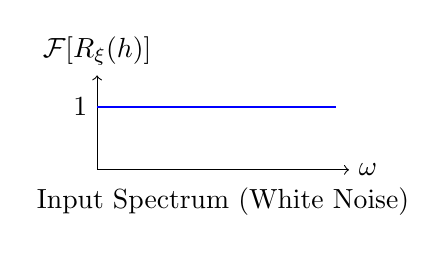
\begin{tikzpicture}[scale=0.8]
        \draw[->] (0,0) -- (4,0) node[right] {$\omega$};
        \draw[->] (0,0) -- (0,1.5) node[above] {$\mathcal{F}[R_{\xi}(h)]$};
        \draw[blue, thick] (0,1) -- (3.8,1) node[right] {};
        \node at (0,1) [left] {$1$};
        \node at (2,-0.5) {Input Spectrum (White Noise)};
    \end{tikzpicture}
    \end{minipage}
    \hfill
    \begin{minipage}{0.45\textwidth}
    \centering
    % Output graph: a Lorentzian shape
    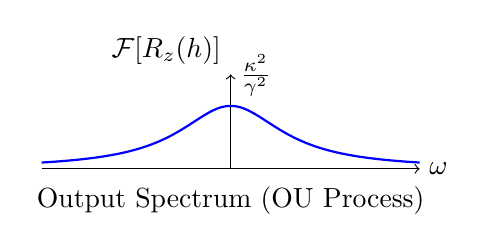
\begin{tikzpicture}[scale=0.8]
        \draw[->] (-3,0) -- (3,0) node[right] {$\omega$};
        \draw[->] (0,0) -- (0,1.5) node[above left] {$\mathcal{F}[R_{z}(h)]$};
        \draw[blue, thick, domain=-3:3, samples=100] plot (\x,{1/(1+\x*\x)});
        \node at (0,1) [above right] {$\frac{\kappa^2}{\gamma^2}$};
        \node at (0,-0.5) {Output Spectrum (OU Process)};
    \end{tikzpicture}
    \end{minipage}
    \caption{Power spectra: input white noise (flat, left) and output OU process (Lorentzian, right).}
\end{figure}

\vspace{-1em}

\subsection{Fokker-Planck equation for Ornstein-Uhlenbeck}

Given the Ito equation for the OU process:
$$
    dz = -\gamma z dt + \omega dW
$$
we can find the Fokker-Planck equation. Recalling the general form of the equation for $P(z,t)$:
$$
    \partial_t P = -\partial_z[a(z)P(z,t)] + \frac{1}{2} \partial_z^2 \left[ b(z)^2 P(z,t) \right]
$$
In our case, with $a(z) = -\gamma z$ and $b(z) = \omega$, it becomes:
$$
    \partial_t P = \partial_z(\gamma z P) + \frac{\omega^2}{2} \partial_z^2 P
$$
This equation is not simple to solve, even with the boundary conditions for a probability density:
$$
    P(\pm\infty, t) = 0 \quad \text{and} \quad \int_{\mathbb{R}} P(z, t) dz = 1
$$
These are additional conditions compared to standard PDEs and are usually of great help.

The most tractable approach is to find the stationary solution $P_s(z)$, which is the long-time limit of $P(z,t)$:
$$
    P_s(z) = \lim_{t\to\infty} P(z,t)
$$
In the stationary state, $\partial_t P = 0$, so the equation becomes an ODE:
$$
    0 = \frac{d}{dz}(\gamma z P_s) + \frac{\omega^2}{2} \frac{d^2 P_s}{d z^2}
$$
which we can rearrange to:
$$
    \frac{d^2 P_s}{d z^2} = - \frac{2\gamma}{\omega^2} \frac{d}{dz}(z P_s)
$$
Integrating once with respect to $z$, we obtain:
$$
    \frac{d P_s}{dz} = C - \frac{2\gamma}{\omega^2} z P_s(z)
$$
The boundary conditions require that $P_s(z) \to 0$ and consequently $P_s'(z) \to 0$ as $z \to \pm\infty$. For this to hold, the integration constant $C$ must be zero. This leaves us with a first-order linear ODE:
$$
    \frac{dP_s}{dz} = - \frac{2\gamma}{\omega^2} z P_s(z)
$$
The solution is a Gaussian function, which is consistent with the properties of the Ornstein-Uhlenbeck process:
$$
    P_s(z) = A e^{-\frac{\gamma}{\omega^2}z^2}
$$
This is nothing other than a Gaussian with $\mu = 0$ and $\sigma^2 = \omega^2/2\gamma$, with $A$ a constant required for normalization, namely
$$
A = \frac{1}{\sqrt{2\pi\sigma^2}}
$$

If we now consider the unperturbed system $\dot{z} = -\gamma z$, we see that the solution tends to $0$ for long times and, since it is deterministic, we obviously have
$$
P^{\mathrm{DET}}_s(z) = \delta(z)
$$
which is consistent with the perturbed case. In fact, the only equilibrium point of the deterministic case is $0$, which turns out to be the center of the Gaussian we found. Therefore, for long times, in the perturbed case, the solution will oscillate around $0$.

\section{The Ginzburg-Landau Model}

We now move from the monostable Ornstein-Uhlenbeck process to a more complex and interesting class of systems: bistable systems. These are systems that possess two stable equilibrium states. The simplest and most iconic model for such a system is the \textbf{Ginzburg-Landau equation}.

\subsubsection{The Deterministic Model}

The deterministic Ginzburg-Landau model describes the dynamics of a particle in a "double-well" potential. The equation of motion is given by:
$$
\dot{x} = x - x^3 = x(1-x)(1+x)
$$
This system has three equilibrium points, found by setting $\dot{x} = 0$:
$$
x_L = -1, \quad x_C = 0, \quad x_R = +1
$$
A simple stability analysis reveals the nature of these points:
\begin{itemize}
    \item $x_L = -1$ and $x_R = +1$ are \textbf{locally asymptotically stable}. If the system starts near one of these points, it will converge to it.
    \item $x_C = 0$ is an \textbf{unstable} equilibrium. If the system starts at this point, any infinitesimal perturbation will cause it to move away towards either $x_L$ or $x_R$.
\end{itemize}

The force $F(x) = x - x^3$ can be derived from a potential $U(x)$ where $F = -dU/dx$:
$$
U(x) = -\frac{x^2}{2} + \frac{x^4}{4}
$$
This potential has a characteristic "double-well" shape, where the stable equilibria $x_L$ and $x_R$ correspond to the minima (the "wells") of the potential, and the unstable equilibrium $x_C=0$ corresponds to the local maximum (the "barrier") between them.

If the initial condition $x(0)$ is drawn from a probability distribution $\theta(x)$, the long-term behavior of the system is deterministic. Any trajectory with $x(0) > 0$ will end up at $x_R = +1$, and any with $x(0) < 0$ will end up at $x_L = -1$. The stationary PDF will therefore consist of two Dirac delta peaks at the stable equilibria, with weights determined by the initial probability of being on either side of the unstable point:
$$
\lim_{t\to\infty} \rho(x,t) = A_R \delta(x-1) + A_L \delta(x+1)
$$
where $A_R = \text{Pr}(x_0>0)$ and $A_L = \text{Pr}(x_0<0)$.

\subsubsection{Stochastic Perturbations of the Model}

Now, let's add a stochastic white noise force to the system:
$$
\dot{x} = x - x^3 + \omega\xi(t) \quad \text{or} \quad dx = (x-x^3)dt + \omega dW_t
$$
This is a case of additive noise perturbing a conservative force. As we derived previously, the stationary probability distribution $P_s(x)$ for such a system is given by the Boltzmann distribution:
$$
P_s(x) = C \exp\left(-\frac{2}{\omega^2}U(x)\right)
$$
Substituting the Ginzburg-Landau potential $U(x) = -x^2/2 + x^4/4$, we get:
$$
P_s(x) = C \exp\left(-\frac{2}{\omega^2}\left(-\frac{x^2}{2} + \frac{x^4}{4}\right)\right) = C \exp\left(\frac{x^2}{\omega^2} - \frac{x^4}{2\omega^2}\right)
$$
where $C$ is a normalization constant. The shape of this distribution is fundamentally controlled by the noise intensity $\omega$.

% picture ?

The relationship between the potential $U(x)$ and the stationary PDF $P_s(x)$ is clear:
\begin{itemize}
    \item The stable equilibria of the deterministic system (minima of $U(x)$) become the \textbf{modes} (peaks) of the stationary PDF.
    \item The unstable equilibrium (maximum of $U(x)$) becomes the \textbf{antimode} (trough) of the stationary PDF.
\end{itemize}

The noise intensity $\omega$ determines how closely the system is confined to these potential wells:
\begin{itemize}
    \item \textbf{Weak Noise ($\omega \ll 1$):} The distribution $P_s(x)$ is sharply bimodal, with two distinct peaks centered around $x=-1$ and $x=+1$. The probability of finding the particle near the unstable point $x=0$ is extremely low. The system will exhibit small stochastic fluctuations around one of the two stable states for very long periods.
    \item \textbf{Strong Noise ($\omega \gg 1$):} The noise provides enough energy for the particle to easily cross the potential barrier between the two wells. The two peaks in the PDF broaden and merge, and the distribution becomes unimodal, centered at $x=0$. For very large $x$, the $x^4$ term still dominates, so the probability $P_s(x)$ must decay to zero.
\end{itemize}

\begin{minipage}{0.48\textwidth}
    \begin{figure}[H]
    \centering
    % PDF for small omega
    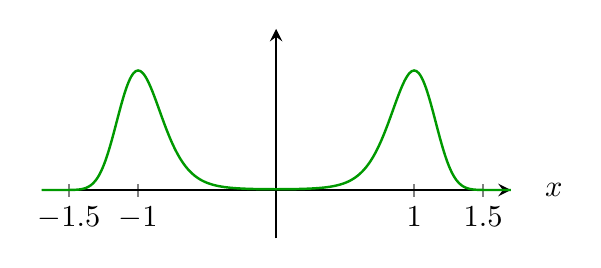
\begin{tikzpicture}[scale=1.1]
        \begin{axis}[
            width=7cm,
            height=4cm,
            domain=-1.7:1.7,
            samples=200,
            axis lines=middle,
            xlabel={$x$},
            ylabel={},
            xtick={-1.5,-1,0,1,1.5},
            ytick=\empty,
            ymin=-60, ymax=200,
            xmin=-1.7, xmax=1.7,
            every axis y label/.style={at={(ticklabel* cs:1.05)},anchor=south},
            every axis x label/.style={at={(ticklabel* cs:1.05)},anchor=west},
            axis line style=thick,
            tick style={thick}
        ]
        % Small omega: sharply bimodal
        \addplot[domain=-1.7:1.7, smooth, thick, color=green!60!black] {exp(x^2/0.1 - x^4/0.2)};
        \end{axis}
    \end{tikzpicture}
    \caption{PDF (non normalized) for small $\omega$}
    \end{figure}
\end{minipage}
\hfill
\begin{minipage}{0.48\textwidth}
    \begin{figure}[H]
    \centering
    % PDF for large omega
    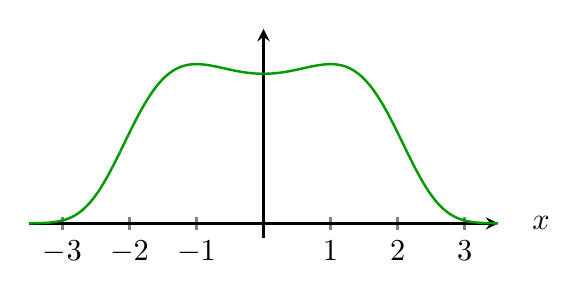
\begin{tikzpicture}[scale=1.1]
        \begin{axis}[
            width=7cm,
            height=4cm,
            domain=-3.5:3.5,
            samples=200,
            axis lines=middle,
            xlabel={$x$},
            ylabel={},
            xtick={-3,-2,-1,0,1,2,3},
            ytick=\empty,
            ymin=-0.1, ymax=1.3,
            xmin=-3.5, xmax=3.5,
            every axis y label/.style={at={(ticklabel* cs:1.05)},anchor=south},
            every axis x label/.style={at={(ticklabel* cs:1.05)},anchor=west},
            axis line style=thick,
            tick style={thick}
        ]
        % Large omega: broad, unimodal
        \addplot[domain=-3.5:3.5, smooth, thick, color=green!60!black] {exp(x^2/8 - x^4/16)};
        \end{axis}
    \end{tikzpicture}
    \caption{PDF (non normalized) for large $\omega$}
    \end{figure}
\end{minipage}

\vspace{0.5em}

This "inheritance" of stability properties from the deterministic potential to the modes of the stationary PDF is a key feature of systems with additive noise. As we will see, this direct correspondence breaks down in the presence of multiplicative noise.

\begin{observationblock}[Stochastic Miultistability]
    It is possible to say that after a very long period of time, also the first case we could see that the system moves from one peak to the other. This is due to the fact that the system is not stable and we have a non-zero probability of moving from one peak to the other. 
\end{observationblock}

\section{Multiplicative Noise}

While additive noise provides a good model for systems perturbed by external forces, many real-world systems feature fluctuations whose intensity depends on the state of the system itself. This leads to the concept of \textbf{multiplicative noise}, which can induce much richer and more complex behaviors than its additive counterpart.

\subsubsection{General SDE and Stationary Fokker-Planck Equation}

Consider a system governed by a parameter $p$. The simplest case is when it is possible to write the field in the form
$$
\dot{x} = b(x) + p \hat{g}(x)
$$
that is, with linear dependence on the parameter considered. The parameter $p$ is usually influenced by the external world, so in some cases it is possible for it to become stochastic. We can then describe a stochastic $p$ as
$$
p \to p + \alpha \xi(t)
$$
Substituting, we obtain
$$
\dot{x} = b(x) + p \hat{g}(x) + \hat{g}(x) \alpha \xi(t)
$$
We can then group the stochastic terms, obtaining
$$
\dot{x} = f(x) + g(x) \xi(t)
$$
The Fokker-Planck equation for the general case is:
$$
\frac{\partial \rho}{\partial t} = - \frac{\partial}{\partial x} [f(x) \rho] + \frac{\partial^2}{\partial x^2} \left[ \frac{g(x)^2}{2} \rho \right]
$$
So far, we have only considered cases where $g(x)$ is constant. Here, however, we are dealing with the most general version of what we have seen so far. The boundary conditions remain the same as before, and as usual, we analyze the stationary case. We have:
$$
\frac{d}{dx} \left[ \frac{g(x)^2}{2} P_s(x) \right] = f(x)P_s(x)
$$
This is a first-order ODE that can be solved for $P_s(x)$. Let's define an auxiliary function $Q(x) = \frac{g(x)^2}{2} P_s(x)$. The equation becomes:
$$
\frac{dQ}{dx} = f(x) \frac{2}{g(x)^2} Q(x)
$$
This is a standard linear ODE of the form $Q'(x) = a(x)Q(x)$, whose solution is $Q(x) = C e^{A(x)}$, where $A(x) = \int a(s)ds$. Applying this, we find:
$$
Q(x) = C \exp\left( \int \frac{2f(s)}{g(s)^2} ds \right)
$$
Substituting back $P_s(x) = \frac{2}{g(x)^2}Q(x)$, we arrive at the general solution for the stationary PDF:
$$
P_s(x) = \frac{C'}{g(x)^2} \exp\left( \int^x \frac{2f(z)}{g(z)^2} dz \right)
$$
where $C'$ is a normalization constant. Let's remark that, being a probability density, the integral of $P_s(x)$ over the entire state space must be equal to one.

We can distinguish two cases:
\begin{itemize}
    \item If the integral exists (is finite), then everything is fine and we can calculate $C$ to normalize $P_s(x)$.
    \item If instead the integral is infinite, we can only find a formal solution that has no physical meaning: in this case it is necessary to study the steady state directly starting from the SDE.
\end{itemize}

\subsection{Noise-Induced Transitions}

In the case of additive noise ($g(x) = \text{const}$), the extrema of the stationary PDF $P_s(x)$ coincide with the equilibria of the deterministic system (where $f(x)=0$). With multiplicative noise, this simple correspondence breaks down.

Recall the following identity, which will be useful for manipulating the stationary distribution:
$$
\dfrac 1{g^2(x)} = e^{-\ln g^2(x)} = e^{-2 \ln g(x)}
$$

Using this, we can rewrite the stationary probability density function in a more transparent exponential form:
$$
P_s(x) = 2 C \exp \left\{
    - 2 \log (g(x)) + \int_\alpha^x \dfrac{2 f(s)}{g^2(s)} ds
\right\}
$$
This highlights how both the noise amplitude $g(x)$ and the drift $f(x)$ contribute to shaping the stationary distribution.

To investigate the location of the extrema of $P_s(x)$, we differentiate with respect to $x$. Applying the chain rule to the exponent, we obtain:
$$
P_s'(x) = 2 C \exp \left\{
    - 2 \dfrac{g'(x)}{g(x)} + \dfrac{2 f(x)}{g^2(x)}
    \right\}
$$
This expression will allow us to determine where the stationary distribution attains its maxima and minima, as these correspond to the points where $P_s'(x) = 0$.

To find the extrema of $P_s(x)$, we must find where its derivative is zero, $P_s'(x)=0$. After some algebraic manipulation of the general solution, this condition simplifies to:

$$
f(x) \ge g(x)g'(x)
$$

This time, unfortunately, we no longer have the close connection we had before; everything now depends on $\alpha$ and on the structure of $g(x)$. In fact, I can rewrite the relation as

$$
f(x) \geq \alpha^2 g'(x) g(x)
$$

This remarkable result shows that the modes of the stationary distribution are no longer located at the deterministic equilibria ($f(x)=0$). Instead, their locations are shifted by a term that depends on the noise function $g(x)$ and its derivative.


This phenomenon, discovered by Horsthemke and Lefever in the 1970s, is called a \textbf{Noise-Induced Transition (NIT)}. It means that by simply varying a parameter that controls the noise intensity, new extrema can appear in the PDF that were completely absent in the unperturbed deterministic system.

Before the discovery of NITs, it was commonly believed that noise could only act in two ways:
\begin{itemize}
    \item In unimodal systems, it creates a "cloud" of fluctuations around the single deterministic equilibrium.
    \item In multimodal systems, it can cause "jumps" between the existing deterministic equilibria.
\end{itemize}
NITs showed that noise can play a much more constructive role, inducing oscillations and creating entirely new states that are not present in the unperturbed deterministic system.

\begin{exampleblock}[Noise-Induced Bifurcation in Gene Expression]
Consider a simple model for protein production, where a protein X acts as its own transcription factor. The production rate is $Q(x)$ and the degradation rate is $dx$.
$$
\dot{x} = Q(x) - dx
$$
A common form for $Q(x)$ that models self-regulation is:
$$
Q(x) = R + K\frac{x^2}{K_d + x^2}
$$
where $R$ is a basal production rate and the second term is a Hill function describing feedback. The deterministic system is:
$$
\dot{x} = \underbrace{R + K\frac{x^2}{K_d + x^2} - dx}_{f(x)}
$$
For small degradation rates $d$, this system has a single, globally stable equilibrium point.

Now, suppose the degradation rate $d$ is subject to stochastic fluctuations: $d \to d + \alpha\xi(t)$. The SDE becomes:
$$
dx = \left(R + K\frac{x^2}{K_d + x^2} - dx\right)dt - \alpha x dW_t
$$
Here, the noise is multiplicative, with $g(x) = -\alpha x$, so $g'(x) = -\alpha$. The condition for the extrema of the stationary PDF, $f(x) \ge g(x)g'(x)$, is:
$$
R + K\frac{x^2}{K_d + x^2} - dx \ge (-\alpha x)(-\alpha) = \alpha^2 x
$$
Rearranging gives:
$$
R + K\frac{x^2}{K_d + x^2} \ge (d + \alpha^2)x
$$
Depending on the value of the noise parameter $\alpha$, this algebraic equation can have one or three solutions. This means that by changing the noise intensity, the stationary PDF can transition from being unimodal (with one peak) to bimodal (with two peaks), even though the underlying deterministic system only had one equilibrium point. This is a classic example of a noise-induced transition: the noise itself creates new, stable macroscopic states for the system.
\end{exampleblock}

\newpage

\section{Perturbation of the Logistic Growth Model}
Let's revisit the logistic growth model, which serves as another prime example of how multiplicative noise can fundamentally alter a system's behavior. We start with the deterministic logistic equation:
$$
\dot{z} = r_1 z - r_2 z^2
$$
Through a linear change of variables $x = r_2 z$, we can adimensionalize the equation to a simpler form:
$$
\dot{x} = r x - x^2
$$
Now, we introduce stochasticity by perturbing the intrinsic growth rate, $r \to r + \omega\xi(t)$. This leads to the corresponding Itô equation with multiplicative noise:
$$
dx = (r x - x^2)dt + \omega x dW_t
$$
This defines our drift and diffusion coefficients as $f(x) = r x - x^2$ and $g(x) = \omega x$.

The stationary Fokker-Planck equation for this system is:
$$
\frac{d}{dx} \left[ \frac{g(x)^2}{2} P_s(x) \right] = f(x)P_s(x)
$$
Substituting our specific $f(x)$ and $g(x)$ gives:
$$
\frac{d}{dx} \left[ \frac{\omega^2 x^2}{2} P_s(x) \right] = (r x - x^2)P_s(x)
$$

To solve this differential equation, we can use the substitution method. Let $Q = x^2 P_s$, then:
$$
Q' = \frac{2r-x}{\omega^2 x} Q
$$
This can be rewritten as:
$$
\frac{dQ}{Q} = \frac{2r-x}{\omega^2 x} dx = \left[\frac{2r}{\omega^2 x} - \frac{1}{\omega^2}\right] dx
$$
Integrating both sides:
$$
\ln Q = \frac{2r}{\omega^2} \ln x - \frac{x}{\omega^2} + C
$$
Taking the exponential:
$$
Q(x) = A \exp\left[\frac{2r}{\omega^2} \ln x - \frac{x}{\omega^2}\right] = A x^{\frac{2r}{\omega^2}} e^{-\frac{x}{\omega^2}}
$$
Since $Q = x^2 P_s$, we obtain:
$$
P_s(x) = \frac{Q(x)}{x^2} = A x^{\frac{2r}{\omega^2}-2} e^{-\frac{x}{\omega^2}}
$$
where $A$ is a normalization constant.


A crucial step is to check whether this candidate solution is a valid, normalizable probability distribution. The integral $\int_0^\infty P_s(x) dx$ must be finite.
$$
\int_0^\infty x^{\frac{2r}{\omega^2}-2} e^{-\frac{2}{\omega^2}x} dx
$$
This is a form of the Gamma function integral, $\int_0^\infty t^{k-1}e^{-t}dt$. For this integral to converge at the lower bound ($x \to 0$), the exponent of $x$ must be greater than -1.
$$
\frac{2r}{\omega^2}-2 > -1 \quad \implies \quad \frac{2r}{\omega^2} > 1 \quad \implies \quad r > \frac{\omega^2}{2}
$$

This is valid only if $r > \omega^2/2$ as we have already seen in the past. If this does not hold, we cannot integrate but what does this actually mean? To understand this, let's return to the SDE:
$$
dx = x(r - x)dt + \omega x dW
$$

Applying now the transformation $y = \psi(x) = \log x$, then $\psi'(x) = x^{-1}$ and $\psi''(x) = -x^{-2}$. Therefore:
$$
dy = \left[\frac{1}{\cancel{x}}x(r - x) - \frac{1}{\cancel{x^2}} \frac{\omega^2 \cancel{x^2}}{2}\right]dt + \omega dW
$$

Therefore, substituting in $y$:
$$
dy = \left[r - \frac{\omega^2}{2} - e^y\right]dt + \omega dW
$$

Integrating then:
$$
y(t) = y_0 + \left(r - \frac{\omega^2}{2}\right)t - \int_0^t e^{y(s)}ds + \omega[W(t) - W(0)]
$$

Notice that the integral term, $-\int_0^t e^{y(s)}ds$, is always negative (since $e^{y(s)} > 0$ for all $s$). 

\begin{itemize}

    \item \textbf{Case 1:} $r < \omega^2/2$

    If $r < \omega^2/2$, the drift term $\left(r - \frac{\omega^2}{2}\right)t$ is negative and dominates for large $t$, while the stochastic term becomes negligible in comparison. As a result, $y(t) \to -\infty$ as $t \to \infty$, which means $x(t) = e^{y(t)} \to 0^+$. In this regime, the probability distribution $P(x, t)$ collapses to a delta function at zero:
$$
    \lim_{t \to \infty} P(x, t) = \delta(x)
$$
This shows that, in this case, the Fokker-Planck equation predicts a stationary solution, but in reality, all probability accumulates at extinction ($x=0$). Thus, the Fokker-Planck approach alone can be misleading for this parameter regime.

    \item \textbf{Case 2:} $r > \omega^2/2$

    On the other hand, when $r > \omega^2/2$, the stationary solution is normalizable and given by:
    $$
        P_s(x) = A x^{\frac{2r}{\omega^2}-2} e^{-\frac{2}{\omega^2}x}
    $$

\end{itemize}


\begin{figure}[H]
    \centering
    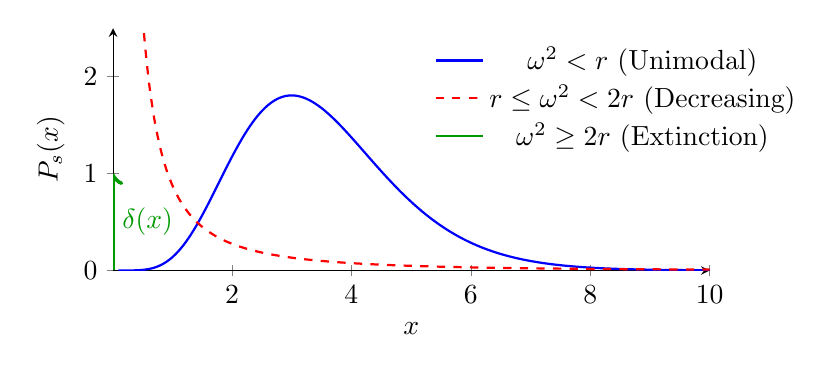
\begin{tikzpicture}
        \begin{axis}[
            scale=0.9,
            width=10cm,
            height=5cm,
            axis lines=left,
            xlabel={$x$},
            ylabel={$P_s(x)$},
            xmin=0.01, xmax=10,
            ymin=0, ymax=2.5,
            legend pos=north east,
            legend style={draw=none, fill=none, xshift=1.5cm},
        ]
        % Case 1: Unimodal PDF (r1 > omega^2)
        \addplot[domain=0.1:10, samples=100, color=blue, thick, smooth] {x^(2*4/1-2)*exp(-2/1*x)};
        \addlegendentry{$\omega^2 < r$ (Unimodal)};
        
        % Case 2: Decreasing PDF (r1 <= omega^2 < 2r1)
        \addplot[domain=0.1:10, samples=100, color=red, thick, smooth, dashed] {x^(2*4/16-2)*exp(-2/16*x)};
        \addlegendentry{$r \le \omega^2 < 2r$ (Decreasing)};
        
        % Case 3: Extinction (delta function, illustrative) - invisible plot for legend
        \addplot[draw=none, color=green!60!black] coordinates {(0,0)};
        \addlegendentry{$\omega^2 \ge 2r$ (Extinction)};
        
        % Case 3: Extinction (delta function, illustrative) - visual representation
        \draw[->, ultra thick, green!60!black] (0.01,0) -- (0.01,1);
        \node[green!60!black, right] at (0, 0.5) {$\delta(x)$};
        
        \end{axis}
    \end{tikzpicture}
    \caption{Noise-Induced Transition in the logistic model.}
\end{figure}


Let us also consider two special cases:
\begin{itemize}
    \item If $\omega^2 = 2r$ (i.e., $2r/\omega^2 = 1$), the stationary distribution simplifies to:
    $$
        P_s(x) = A x^{-1} e^{-\frac{x}{r}}
    $$
    \item If there is no noise, $\omega^2 = 0$, the stationary distribution becomes:
    $$
        P_s(x) = A e^{-\frac{x}{r}}
    $$
    This change has a significant effect on the shape of the stationary distribution. Specifically, when the parameters satisfy
    $$
        \frac{2r}{\omega^2} < 2 \qquad \text{or equivalently} \qquad r < \frac{\omega^2}{2}
    $$
    the distribution $P_s(x)$ is no longer unimodal (with a peak at some $x > 0$), but instead becomes a monotonically decreasing function of $x$. In this regime, the probability density is highest near $x=0$ and decreases for larger $x$, so the system is most likely to be found close to $x=0$.
\end{itemize}


Furthermore, it can be shown that the stationary distribution $P_s(x)$ is normalizable (i.e., its total probability integrates to 1) only if $\omega^2 < 2r$. This is consistent with the more general result discussed in the previous section.